\chapter{Literature review}
\label{sec:lit}
This chapter presents an overview of relevant literature for visual obstacle avoidance.
The review consists of two parts: \autoref{sec:oa} presents an overview of obstacle avoidance systems and their components, paying special attention to the visual detection of obstacles.
Then, \autoref{sec:depthest} takes a closer look at the use of neural networks for depth estimation.

\section{Obstacle Avoidance}
\label{sec:oa}
Practical \acfp{CAS} need to solve a number of subproblems in order to detect and avoid obstacles.
An overview of the tasks involved and possible solutions is given in \cite{Albaker2009,Pham2015}.
In general, a \ac{CAS} contains the following elements:
\begin{itemize}
\item Sensing of the environment
\item Conflict detection
\item Avoidance maneuver: planning and execution
\end{itemize}
The system should have some way to \emph{sense} potential obstacles in its environment.
In this review, sensing will be primarily performed through vision, but other sensors could also be used to detect obstacles.
Communication with other aircraft also falls under this element.
\emph{Conflict detection} is used to decide whether an evasive maneuver should be performed.
It usually requires a method to predict future states of the \ac{UAV} and of detected obstacles or aircraft and a threshold or minimum safe region that should stay free of obstacles.
When the conflict detection indicates that a collision is imminent, an \emph{escape maneuver} has to be performed to avoid this potential collision.
Depending on the method, this maneuver can be performed using simple rules, planned by optimizing some cost function or even performed in collaboration with other aircraft (e.g. \ac{TCAS}).

The elements listed above are typical for the avoidance of other vehicles but can also be used for the avoidance of static obstacles.
In this case, the conflict detection is often skipped or simplified since only the \ac{UAV} itself is moving; instead it is often performed implicitly during the planning of the escape maneuver around the obstacle.

Subsections \ref{sec:sensing} and \ref{sec:avoidance} take a closer look at the sensing of the environment and planning of escape maneuvers.
Conflict detection is not considered for now as this review is primarily aimed at the avoidance of static obstacles.
Subsection \ref{sec:perf} will briefly highlight the literature (or lack thereof) on the performance evaluation of \aclp{CAS}.


\subsection{Sensing}
\label{sec:sensing}
The goal of sensing is to detect and locate nearby obstacles.
The range of sensors that could be used for obstacle detection is large, but a number of these can be ruled out for usage on \acp{UAV} because of their weight or power requirements.
This subsection will focus on the visual detection of obstacles.

The localization of obstacles through vision can be split into two parts: estimation of the bearing towards the obstacle and estimation of the distance.
As long as the obstacle can be reliably found in the image, estimation of the \emph{bearing} is fairly straightforward.
The position of the obstacle in the image is a direct result of its bearing relative to the camera and this relation can be inverted.

Estimation of the \emph{distance} towards the obstacle is more complicated.
Since the obstacle is projected onto the image plane, the depth information is lost.
Other cues need to be used to estimate the distance towards the obstacle.
These cues can be broadly split into three categories:
\begin{itemize}
\item Stereo vision
\item Optical flow
\item Appearance
\end{itemize}
Stereo vision uses two images taken \emph{at the same time} from different locations, optical flow uses two images taken \emph{at different times} and appearance is based on \emph{single} images.
The next subsections take a closer look at these depth estimation methods.




\subsubsection{Stereo vision}
\begin{figure}
\centering
\input{images/stereo.pdf_tex}
\caption{Stereo vision uses the disparity $d$ to estimate the depth $z$ towards obstacles. The camera baseline $B$ and focal length $f$ are constant and obtained through calibration.}
\label{fig:stereo}
\end{figure}

Stereo vision uses images taken at the same time from different viewpoints to estimate depth.
The difference in viewpoints causes the obstacle to appear in different positions in the images.
The difference in these positions -- the \emph{disparity} -- is inversely related to the depth of the object.

An example of depth estimation using stereo vision is shown in \autoref{fig:stereo} for an obstacle at distance $z$ observed using a stereo camera with focal length $f$ and baseline $B$.
Using equal triangles, the disparity of the obstacle is:
\begin{align}
d &= B \ f \ z^{-1}
\end{align}
This equation can be solved for $z$ to find a distance estimate $\hat z$ given a disparity $d$:
\begin{align}
\hat z &= B \ f \ d^{-1}
\end{align}
The camera parameters $B$ and $f$ are found beforehand through calibration.

The main challenge of stereo vision is to find this disparity; it is often difficult to find out which pixels in the images belong to the same point in the world.
A first way to categorize stereo vision algorithms is to make a distinction between sparse and dense algorithms.
\emph{Sparse} algorithms estimate the disparity of a small number of highly recognizable points in the images.
The disparity accuracy tends to be good as these points are easy to match, but because only a small number of points is considered  the resulting depth map can contain large holes, especially in environments with little texture.
Sparse stereo algorithms are therefore a poor choice for obstacle detection, but they sometimes appear as part of \ac{VO} or \ac{SLAM} algorithms.
\emph{Dense} algorithms, on the other hand, estimate the depth for the entire image.
They should therefore be able to estimate the distance towards all obstacles in view.

\begin{figure}
\centering
\begin{subfigure}[b]{0.9\textwidth}
\centering
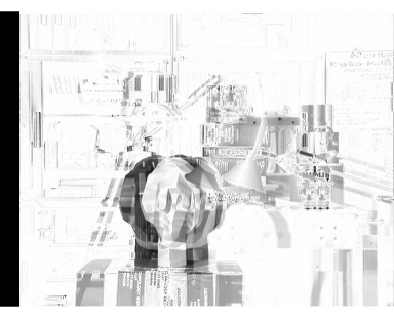
\includegraphics[width=0.3\textwidth]{cost_19.png}
~
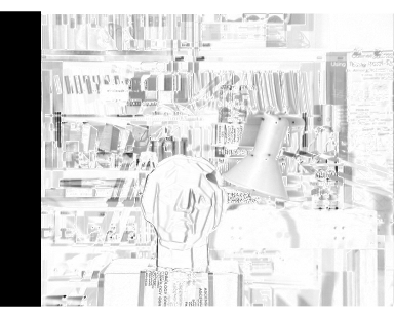
\includegraphics[width=0.3\textwidth]{cost_40.png}
~
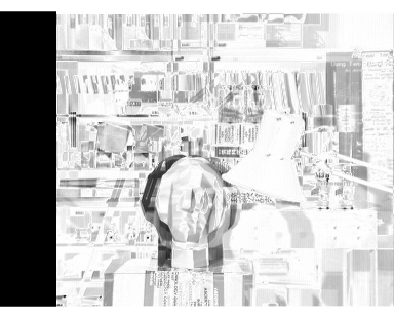
\includegraphics[width=0.3\textwidth]{cost_55.png}
\caption{\emph{Matching cost computation}. The matching cost is calculated per pixel for all disparities under consideration. In this example the pixel difference is used as matching cost. Shown are difference images at three different disparities, where white indicates a low matching cost and black a high cost. In the left image, the disparity is roughly equal to the true disparity of the background: the background has a low matching cost (white). In the middle image, the disparity is close to that of the head; in the right image it is close to that of the lamp.}
\end{subfigure}

\begin{subfigure}[b]{0.9\textwidth}
\centering
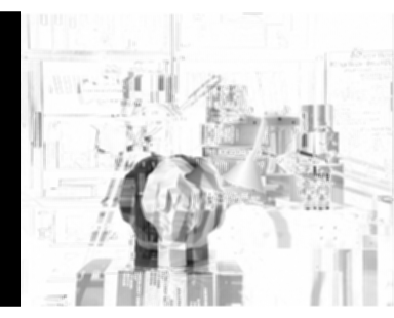
\includegraphics[width=0.3\textwidth]{aggr_19.png}
~
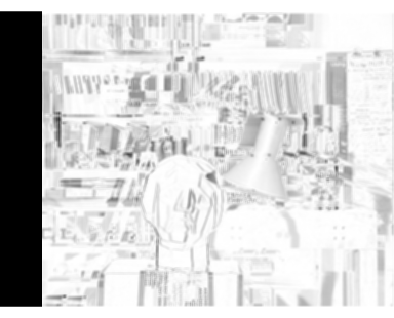
\includegraphics[width=0.3\textwidth]{aggr_40.png}
~
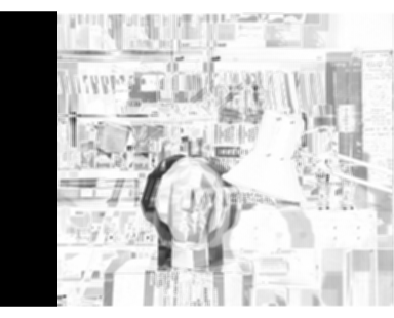
\includegraphics[width=0.3\textwidth]{aggr_55.png}
\caption{\emph{Cost aggregation}. Sometimes individual pixels can be hard to match. In this case, information on neighboring pixels can make the matching task easier. In this example, the matching cost images are convolved with a $3\times 3$ averaging filter to take nearby pixels into account.}
\end{subfigure}

\begin{subfigure}[b]{0.9\textwidth}
\centering
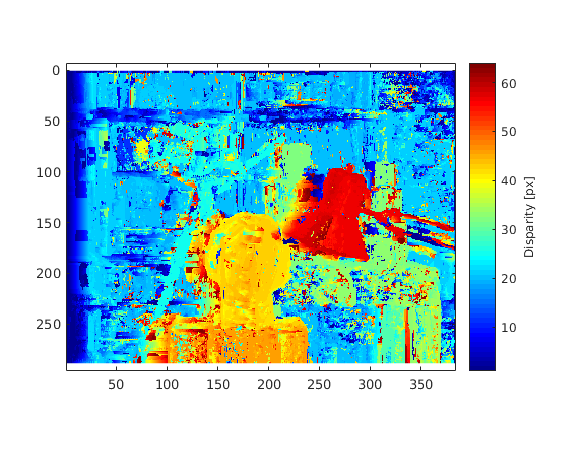
\includegraphics[width=0.4\textwidth]{disp.png}
\caption{\emph{Disparity optimization}. Using the aggregated matching cost, the per-pixel disparity can be found through optimization. In this example, the per-pixel argmax over the disparities is used. This is a form of \emph{local} optimization as the pixel disparities can be found independently.}
\end{subfigure}

\begin{subfigure}[b]{0.9\textwidth}
\centering
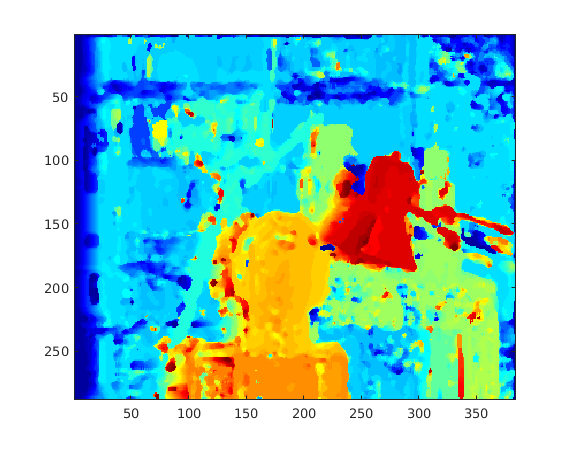
\includegraphics[width=0.35\textwidth]{disp_ref.png}
\caption{\emph{Disparity refinement}. Post-processing is used to clean up the disparity map from the previous step. In this example, a median filter is used to remove outliers.}
\end{subfigure}
\caption{Example of the \emph{block matching} stereo algorithm broken down into the four steps described by \citet{Scharstein2002}.}
\label{fig:stereo_example}
\end{figure}

In \cite{Scharstein2002}, \citeauthor{Scharstein2002} present an extensive taxonomy of dense stereo vision algorithms.
According to the authors, most dense stereo vision algorithms perform the following steps to find a disparity map:
\begin{enumerate}
\item Matching cost computation
\item Cost aggregation
\item Disparity optimization
\item Disparity refinement
\end{enumerate}
An example of these four steps is shown in \autoref{fig:stereo_example} for the \emph{block matching} algorithm.

An important distinction can be made between global and local algorithms, which differ in the way the disparity optimization is performed.
\emph{Global} algorithms try to optimize a single cost function that depends on all pixel disparities.
These algorithms can produce accurate depth maps even for scarcely textured scenes, but tend to be slower than local algorithms.
\emph{Local} algorithms independently optimize the disparities of pixels or small regions.
These algorithms are easier to parallelize and typically faster, but less accurate.

\medskip

An in-depth review of stereo vision methods is out of scope for this report.
While it is important to understand the working of stereo vision algorithms, their run-time performance and accuracy are perhaps more relevant for their use on \acp{UAV}.
These are difficult to predict from first principles and are instead measured on benchmarks, of which the Middlebury Stereo benchmark\footnote{\url{http://vision.middlebury.edu/stereo/}} \cite{Scharstein2002} and the KITTI Stereo benchmark\footnote{\url{http://www.cvlibs.net/datasets/kitti/eval_scene_flow.php?benchmark=stereo}} \cite{Menze2015} are commonly-used examples.

In \cite{Tippetts2016}, \citeauthor{Tippetts2016} perform an extensive review of stereo vision algorithms for resource-limited systems.
The authors collected run-time and accuracy measurements for a large number of algorithms and use these to produce scatterplots of their performance.
Where possible, the run-times were normalized based on the hardware for which they were reported.
The article provides an excellent starting point for the selection of stereo algorithms, its only downside being that it was written in 2012 and that it is therefore not fully up-to-date.

A similar review was performed for this literature study, so that algorithms published after 2012 could also be included.
Run-time and accuracy measures were obtained from the Middlebury and KITTI benchmarks.
Run-time figures were not normalized, as the majority of methods are evaluated on similar platforms (CPU-based methods on an unspecified \SI{2.5}{\giga\Hz} processor, GPU-based methods on an NVIDIA Titan X).
The main focus of this comparison is on algorithms for which code is publicly available.
The results are shown in \autoref{fig:stereo_benchmark}.

The following conclusions are drawn from these results: first of all, there exist close-to-optimal stereo vision algorithms for which code is publicly available.
This means that it is not necessary to write an own implementation of a state-of-the-art algorithm.
Secondly: from the CPU-based methods, \acs{ELAS} \cite{Geiger2011} and \acs{SGM}/\acs{SGBM} variants \cite{Hirschmuller2008} are still among the best performers.
The inclusion of \acs{SGBM} in OpenCV makes this an ideal algorithm for initial development.
Thirdly: the use of a GPU can significantly increase performance, mainly in terms of accuracy.
However, it is currently unclear how this performance improvement weighs up against the increase in weight and power consumption of such a platform.
The \SI{250}{\W} required by the NVIDIA Titan X is quite high for a \ac{UAV}, and the performance benefit seen in the benchmarks might be significantly smaller on an embedded GPU.

\begin{figure}
\centering
\begin{subfigure}[t]{0.45\textwidth}
\centering
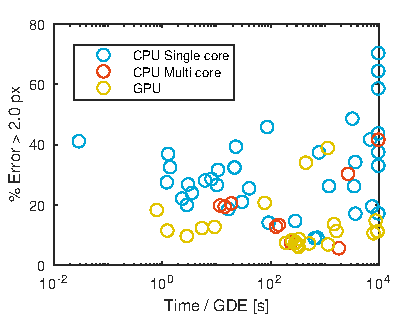
\includegraphics{middlebury_stereo_platform.pdf}
\caption{Platforms and performance on the Middlebury benchmark.}
\label{fig:mid_platform}
\end{subfigure}
~
\begin{subfigure}[t]{0.45\textwidth}
\centering
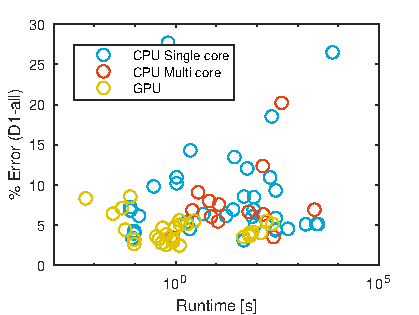
\includegraphics{kitti_stereo_platform.pdf}
\caption{Platforms and performance on the KITTI benchmark.}
\label{fig:kitti_platform}
\end{subfigure}

\begin{subfigure}[t]{0.45\textwidth}
\centering
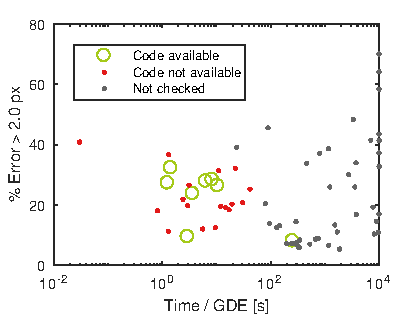
\includegraphics{middlebury_stereo_code.pdf}
\caption{Code availability on the Middlebury benchmark.}
\end{subfigure}
~
\begin{subfigure}[t]{0.45\textwidth}
\centering
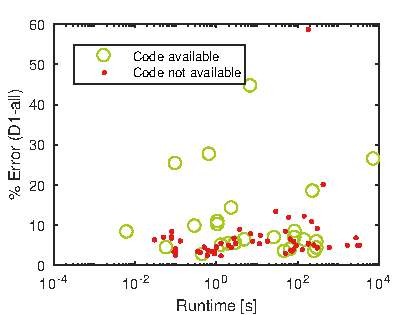
\includegraphics{kitti_stereo_code.pdf}
\caption{Code availability on the KITTI benchmark.}
\end{subfigure}

\begin{subfigure}[t]{0.45\textwidth}
\centering
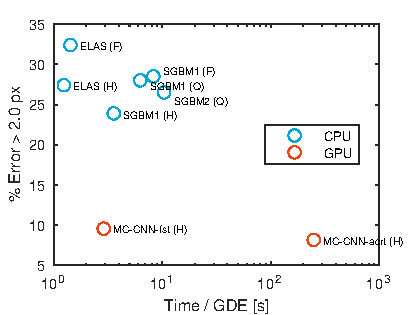
\includegraphics{middlebury_stereo_detail.pdf}
\caption{Best performing methods on the Middlebury benchmark for which code is available.}
\end{subfigure}
~
\begin{subfigure}[t]{0.45\textwidth}
\centering
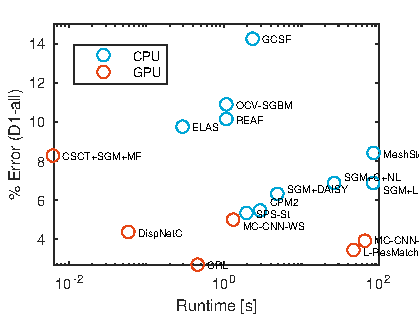
\includegraphics{kitti_stereo_detail.pdf}
\caption{Best performing methods on the KITTI benchmark for which code is available.}
\end{subfigure}
\caption{Scatterplots of accuracy versus runtime performance on the Middlebury and KITTI stereo vision benchmarks. Data obtained on 27/11/2017.
\emph{a, b}: Methods running on the GPU tend to perform better than those running on the CPU. On the Middlebury benchmark they perform better in terms of accuracy, while on the KITTI benchmark they also outperform CPU methods in terms of runtime -- perhaps because runtime performance is more important for automotive applications than for the static pictures of Middlebury.
\emph{c, d}: While code is not available for every method, there are enough close-to-optimal algorithms for which source code has been published.
\emph{e, f}: These methods should be considered first when choosing a stereo vision algorithm, as they perform well and their code is publicly available. Popular choices are \acs{ELAS} \cite{Geiger2011} and \acs{SGM}/\acs{SGBM} \cite{Hirschmuller2008}; the latter is also included in OpenCV.}
\label{fig:stereo_benchmark}
\end{figure}

\medskip

On a higher level, stereo vision has the advantage over other depth cues that its depth estimate is based on the \emph{baseline} between the two cameras.
This is an advantage because the baseline is constant and easy to measure or calibrate.
In comparison, the distance between successive images for optical flow is often unknown; it has to be estimated and therefore leads to more uncertainty in the distance estimate.
Appearance cues have a similar disadvantage, the size of certain cues in the environment is not exactly known, also leading to uncertainty in the depth estimate.

Stereo vision also has limitations.
First of all it requires two or more cameras.
The resulting weight will be larger for this setup than for depth estimation based on optical flow or appearance cues.

Secondly, the range of stereo vision is limited, although not as badly as commonly thought \cite{Pinggera2014}.
As the distance to obstacles increases, the disparity decreases inversely (see \autoref{fig:stereo_lim}).
This means that for far-away objects the disparity hardly changes with distance.
As a result, the sensitivity to measurement errors $\md \hat z / \md d$ increases with distance until it becomes impractically large:
\begin{align}
\frac{\md \hat z}{\md d} &= -B \ f \ d^{-2} \\
&= - \frac{z^2}{B\ f}
\end{align}
This growing uncertainty limits the maximum range of stereo vision.
The disparity errors are the result of incorrect matching of pixels in the input images and are typically independent of distance.
If the stereo algorithm only searches for discrete disparities, these errors will be in the order of \SI{0.5}{\px} at best.
Stereo algorithms for long-range distances therefore need to estimate subpixel disparities.
According to \citeauthor{Pinggera2014}, it is possible to reach a consistent error limit of \SI{0.1}{\px} under real-world conditions \cite{Pinggera2014}.
The sensitivity to measurement errors can also be reduced by increasing the baseline $B$ or focal length $f$ of the cameras.

Finally, the matching of features between the input images is often a weak point of stereo vision.
As a result, it may perform badly with the following obstacles: textureless surfaces, finely or repetitively textured surfaces, textures oriented parallel to the baseline, reflections and transparency.
Furthermore, depending on the algorithm, slanted surfaces and occlusions can be problematic.

\begin{figure}
\centering
\begin{subfigure}[t]{0.45\textwidth}
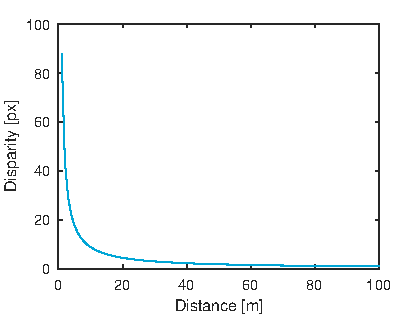
\includegraphics{stereo_disparity.pdf}
\caption{Disparity vs. distance. As the distance increases, the disparity converges to zero. For far-away objects the disparity hardly changes with distance anymore.}
\end{subfigure}
~
\begin{subfigure}[t]{0.45\textwidth}
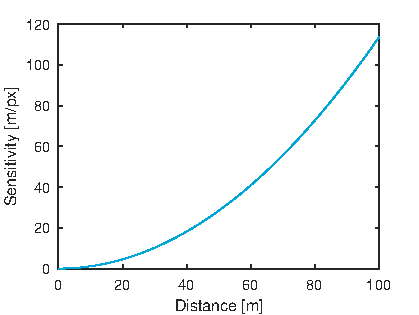
\includegraphics{stereo_sensitivity.pdf}
\caption{Sensitivity vs. distance. The sensitivity is defined as $-\md z / \md d$, i.e. the distance error for a \SI{1}{\px} error in the disparity estimate.}
\end{subfigure}
\caption{Maximum range of stereo vision. As the distance increases, the sensitivity to stereo matching errors increases quadratically. Example plots generated for a camera with baseline $B=\SI{20}{\centi\meter}$ and focal length $f=\SI{400}{\px}$. Best-case disparity errors are in the order of \SI{0.5}{\px} to \SI{0.1}{\px} \cite{Pinggera2014} depending on the algorithm.}
\label{fig:stereo_lim}
\end{figure}





\subsubsection{Optical flow}
\begin{figure}
\centering
\input{images/flow.pdf_tex}
\caption{Optical flow for forward motion. The image position $u$ of an obstacle located at $(x, z)$ changes as the \ac{UAV} moves forward with a velocity of $-\dot z$.}
\label{fig:optical_flow}
\end{figure}

Optical flow tracks the movement of image features over time.
In a static environment, the shift of these features depends on the movement of the camera and the distance to the features; in general, features further away from the camera will move less than those that are nearby.
If the movement of the camera is known, the distance to the features can be obtained.
When only the rotation is known the distance cannot be found; however it is still possible to estimate the time-to-contact, which is sufficient for some forms of obstacle avoidance.

\autoref{fig:optical_flow} shows an example of optical flow and its use for depth estimation.
The example assumes forward motion\footnote{Optical flow from sideways or vertical motion has slightly different characteristics, but will not be explained here to keep the explanation short. A forward-facing camera is the most relevant example for obstacle avoidance.} at a known velocity without rotation of the camera.
Given the obstacle's position $(x, z)$ and the camera's focal length $f$, its image position $u$ can be found using equal triangles:
\begin{align}
u &= x \ f \ z^{-1}
\end{align}
Taking the time derivative produces the instantaneous optical flow $\dot u$ of the obstacle or feature:
\begin{align}
\dot u &= -x \ f \ z^{-2} \ \dot z \\
&= - u \ z^{-1} \ \dot z \label{eq:of_udot}
\end{align}
In practice, however, the optical flow is estimated between two images separated by a time interval $\Delta t$. The result is a shift in position $\Delta u$ instead of the flow $\dot u$:
\begin{align}
\Delta u &\approx \dot u \ \Delta t \\
&\approx - u \ z^{-1} \ \dot z \ \Delta t \label{eq:of_deltau}
\end{align}
The depth $\hat z$ can be found by solving this equation for $z$:
\begin{align}
\hat z &= -u \ \dot z \ \Delta t \ \Delta u^{-1} \quad \forall \Delta u \neq 0 \implies \forall u \neq 0
\end{align}
and, if velocity $\dot z$ is not available, the time-to-contact $\tau$ is found using:
\begin{align}
\tau &= \hat z / \dot z \\
&= -u\ \Delta t \ \Delta u^{-1}
\end{align}
Note, however, that from \autoref{eq:of_udot} and \ref{eq:of_deltau} it follows that the flow $\dot u$ and shift $\Delta u$ will be zero in the center of the image where $u$ is zero (the \acl{FoE}).
It is therefore not possible to estimate depth at the Focus-of-Expansion as the result is undefined.

\medskip

The main problem of optical flow is not the estimation of depth but the tracking of features between images.
It is therefore very similar to stereo vision.
The main difference, however, is that stereo vision only searches for matches along one dimension, while optical flow is two-dimensional.
Optical flow is therefore more difficult to compute.

As in stereo vision, a distinction can be made between sparse and dense optical flow algorithms.
\emph{Sparse} algorithms track highly recognizable points, typically corners.
Sparse tracking is frequently found in \ac{VO} or \ac{SLAM}.
Like sparse stereo vision, sparse optical flow is not suitable for obstacle detection as it may leave large holes in the depth map.
\emph{Dense} algorithms estimate optical flow for the complete image and are therefore better suited for obstacle detection.

An overview of optical flow techniques is presented in \cite{Baker2011}.
The survey is similar to \cite{Scharstein2002} in that it breaks down the algorithms into a few key components.
According to \citeauthor{Baker2011}, most dense optical flow algorithms perform a global optimization (i.e. for all pixels at the same time) of the following energy function: $E_\text{data} + \lambda E_\text{prior}$, where the \emph{data term} $E_\text{data}$ follows from the content of the images (similar to the matching cost in stereo vision) and the \emph{prior term} $E_\text{prior}$ encodes assumptions of the flow field such as its smoothness \cite{Baker2011}.
The final component of a dense optical flow algorithm is the \emph{optimization algorithm}.

An in-depth overview of optical flow algorithms is again beyond the scope of this report.
Instead, existing optical flow algorithms are compared by benchmark results.
The results are obtained from \citeay{Baker2011} \cite{Baker2011} (the more up-to-date Middlebury website\footnote{\url{http://vision.middlebury.edu/flow/}} unfortunately does not report run-times) and from the KITTI optical flow 2015 benchmark\footnote{\url{http://www.cvlibs.net/datasets/kitti/eval_scene_flow.php?benchmark=flow}} \cite{Menze2015}.
The results are shown in \autoref{fig:flow_benchmark}.

The KITTI results show that code is available for fast and accurate optical flow estimation on GPUs.
Code for the best performing CPU-based algorithms is not available; SPyNet \cite{Ranjan2016} might be used as an equally fast alternative, but it has a higher error percentage then the best-performing algorithms.
The other CPU-based algorithms for which code is available have run-times larger than one second.
While it may be possible to reduce their run-times by, for instance, lowering the resolution of the images, there is no guarantee that they will run fast enough for practical use in obstacle avoidance.
From the results of \citeay{Baker2011} only FOLKI has a run-time of one second, while the others are in the order of ten seconds or more.


\begin{figure}
\centering
\begin{subfigure}[t]{0.45\textwidth}
\ % No data
\end{subfigure}
~
\begin{subfigure}[t]{0.45\textwidth}
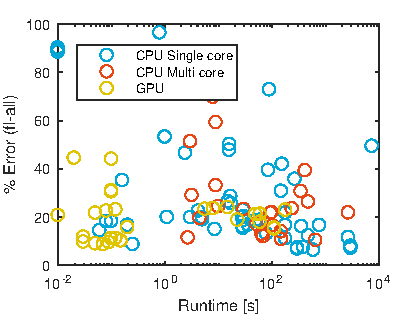
\includegraphics{kitti_flow2015_platform.pdf}
\caption{Platform and performance on the KITTI benchmark.}
\end{subfigure}

\begin{subfigure}[t]{0.45\textwidth}
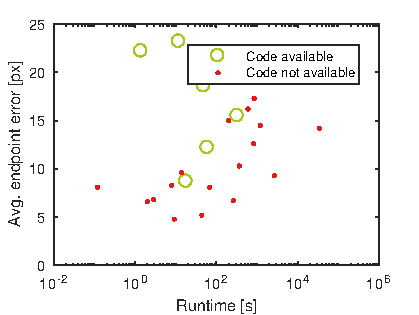
\includegraphics{baker2011_flow_code.pdf}
\caption{Code availability of the methods reviewed in \citeay{Baker2011}.}
\end{subfigure}
~
\begin{subfigure}[t]{0.45\textwidth}
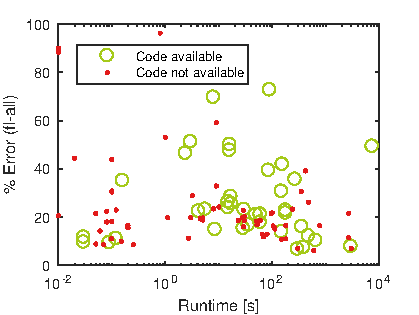
\includegraphics{kitti_flow2015_code.pdf}
\caption{Code availability on the KITTI benchmark.}
\end{subfigure}

\begin{subfigure}[t]{0.45\textwidth}
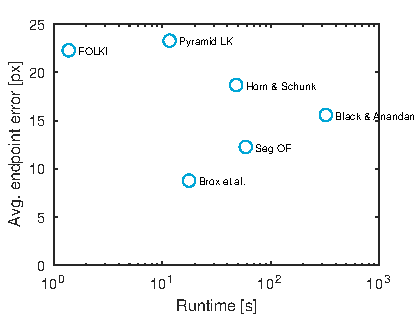
\includegraphics{baker2011_flow_detail.pdf}
\caption{Best performing methods in \citeay{Baker2011} for which code is available.}
\end{subfigure}
~
\begin{subfigure}[t]{0.45\textwidth}
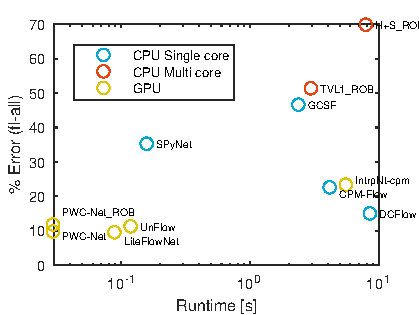
\includegraphics{kitti_flow2015_detail.pdf}
\caption{Best performing methods on the KITTI benchmark for which code is available.}
\end{subfigure}
\caption{Scatterplots of dense optical flow estimation accuracy and run-time performance. Data is obtained from \citeay{Baker2011}~\cite{Baker2011} and the KITTI optical flow 2015 benchmark \cite{Menze2015} (data obtained on 28/08/2018).
\emph{a}: GPU-based methods tend to have lower runtimes and error percentages than CPU-based algorithms. (Platform information is not available for \citeay{Baker2011}).
\emph{b, c}: Of the methods listed in \citeay{Baker2011}, source code is not available for the best performing ones. This is slightly better for the KITTI benchmark.
\emph{d, e}: These are the best performing methods for which code is publicly available. GPU-based methods perform significantly better than CPU-based ones. There is little overlap between \citeay{Baker2011} and KITTI in terms of algorithms, but note that there is a 7-year gap between the two benchmarks. The algorithm by \citeauthor{Brox2004} is included in OpenCV \cite{Brox2004}. For the other methods code is available, but it might take more work to integrate these into research code.}
\label{fig:flow_benchmark}
\end{figure}

\medskip

Compared to stereo vision, the main advantage of optical flow is that it only requires a single camera, which saves weight.
However, optical flow also has a number of disadvantages.
First of all, if a metric depth estimation is required, the velocity of the \ac{UAV} should be known.
Estimation of this velocity is not trivial and uncertainties in this estimate are an additional source of error for depth estimation.

\begin{figure}
\centering
\begin{subfigure}[t]{0.45\textwidth}
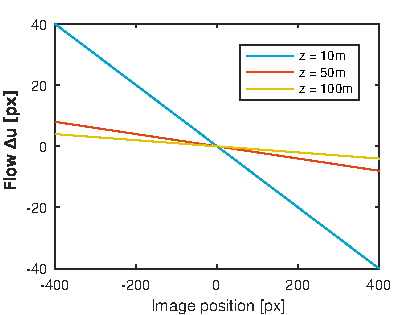
\includegraphics{flow_s1}
\caption{Expected optical flow $\Delta u$ as a function of image position $u$ for three obstacle distances $z$.}
\end{subfigure}
~
\begin{subfigure}[t]{0.45\textwidth}
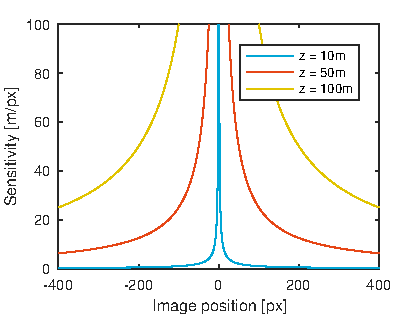
\includegraphics{flow_s2}
\caption{Sensitivity to measurement errors in $\Delta u$ as a function of image position $u$ for three obstacle distances $z$.}
\end{subfigure}

\begin{subfigure}[t]{0.45\textwidth}
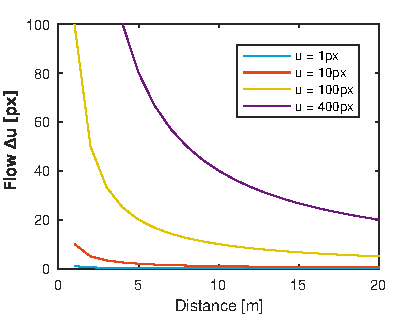
\includegraphics{flow_s3}
\caption{Expected optical flow $\Delta u$ as a function of obstacle distance $z$ for four image positions $u$.}
\end{subfigure}
~
\begin{subfigure}[t]{0.45\textwidth}
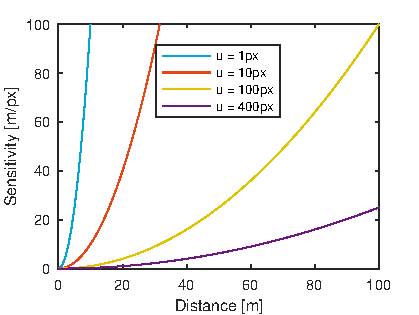
\includegraphics{flow_s4}
\caption{Sensitivity to measurement errors in $\Delta u$ as a function of obstacle distance $z$ for four image positions $u$.}
\end{subfigure}
\caption{Example of expected optical flow and sensitivity to measurement errors in $\Delta u$. Data generated for a camera traveling at \SI{10}{\meter\per\second} with an optical flow algorithm running at \SI{10}{\Hz} ($\Delta t = \SI{0.1}{\s}$). Plot \emph{b} shows that the sensitivity to errors strongly increases near the center of the image and approaches infinity at the \ac{FoE}. Plot \emph{d} shows that obstacles near the \ac{FoE} ($u=\SI{1}{\px}$) can only be detected at short ranges where the sensitivity to measurement errors is low, while the range is significantly larger near the edge of the image ($u=\SI{400}{\px}$).}
\label{fig:of_sensitivity}
\end{figure}

A second problem is that the optical flow approaches zero near the \ac{FoE}.
By definition the \ac{FoE} lies in the direction of travel, exactly the place where obstacles \emph{should} be detected.
Since the flow needs to be inverted to estimate distance, this makes the depth estimate extremely sensitive to measurement errors in shift $\Delta u$.
This is demonstrated with the sensitivity $\md \hat z / \md \Delta u$, i.e. the error in the distance estimate for a \SI{1}{\px} error in $\Delta u$:
\begin{align}
\frac{\md \hat z}{\md \Delta u} &= u \ \dot z \ \Delta t \ \Delta u^{-2} \\
&= \frac{z^2}{\dot z \ u \ \Delta t} \label{eq:of_sensitivity}
\end{align}
For reference, the best average end-point errors in the KITTI optical flow 2012 benchmark\footnote{\url{http://www.cvlibs.net/datasets/kitti/eval_stereo_flow.php?benchmark=flow}} \cite{Geiger2012} lie in the order of \SI{1}{\px}.
The expected flow and sensitivity are shown in \autoref{fig:of_sensitivity} for a drone traveling at \SI{10}{\meter\per\second}.
The conclusion drawn from this figure is that it may be difficult to get an adequate measurement range near the \ac{FoE}, as the sensitivity to measurement errors rapidly increases for $|u|<\SI{100}{\px}$.

\autoref{eq:of_sensitivity} suggests a few ways to reduce the sensitivity to errors.
First of all, the \ac{UAV} can fly faster; this results in larger flow vectors relative to the measurement error.
Secondly, the frame rate can be \emph{reduced}, this will also increase the size of the flow vectors.
Note, however, that there is an upper limit to $\Delta t$ as the resulting $\Delta u$ should remain small enough that features remain in view.
The frame rate should also remain high enough to detect obstacles in time.
Finally, the sensitivity can be reduced by using a higher-resolution camera or a zoom lens, as $u$ will be larger (note that the sensitivity does not depend on the camera's focal length).

The final disadvantage of optical flow is that it requires sufficient texture to match pixels between successive images.
Like stereo vision, it can produce incorrect results for textureless surfaces, finely or repetitively textured surfaces, reflections and transparency.

\medskip

Not mentioned in this review is \emph{scene flow}, the 3D equivalent of optical flow.
The result of scene flow is a 3-dimensional velocity vector for each pixel, together with a depth or disparity.
A review of this field is left for future work.





\subsubsection{Appearance}
\label{sec:appearance}
Unlike stereo vision or optical flow, appearance cues can be found inside a \emph{single} image.
As humans we are already familiar with appearance-based cues because we use them all the time, such as when looking at photographs.
Photographs do not contain disparities since they are flat, nor do they produce optical flow as they do not move.
Still, it is possible to estimate depth from these images; this is the field of \emph{monocular depth estimation}.

`Appearance' is not really a single cue, as is the case for stereo vision which relies entirely on disparities or optical flow which results only from the flow vectors.
Instead, appearance cues are a collection of image features that depend in one way or another on depth.
An extensive treatment of depth cues used by humans can be found in \cite{Gibson1950}.
The following is a non-exhaustive list of appearance cues:
\begin{itemize}
\item Occlusion. Nearby objects cover those further away.
\item Image size of known objects. Using the focal length of the camera, this can be transformed back into a distance estimate.
\item Different image sizes of similar objects. The objects that appear smaller in the image are further away.
\item Perspective. Parallel lines in the environment appear to converge in the image, their distance provides an indication of depth.
\item Vertical image position. Objects that appear higher in the image are further away.
\item Texture gradient. Surface textures will appear more fine-grained if they are further away.
\item Light and shadow. This cue is especially relevant for surface relief. Light typically comes from above, brighter regions are assumed to face upwards.
\item Atmospheric haze. Far-away objects take on a blue-ish tint.
\item Sky segmentation. The sky is infinitely far away.
\end{itemize}
Most of these cues require knowledge about the environment, such as the presence of a flat ground or parallel lines, knowledge about the size of objects, and so on.
This makes appearance-based depth estimation more difficult to implement than stereo vision or optical flow.
If it is even possible to implement some of these cues, this quickly leads to rather ad-hoc solutions.
For this reason, appearance-based cues have seen relatively little use in computer vision until recently.

\medskip

One of the first practical examples of monocular depth estimation for arbitrary outdoor images is \citeauthor{Saxena2006}'s \emph{Make3D} \cite{Saxena2006,Saxena2009}, first published in \citeyear{Saxena2006}.
The system relies on a combination of superpixel segmentation and hand-crafted features.
These are fed into a \ac{MRF} to model the relations between the regions in the image.

The field of monocular depth estimation really took off with the arrival of Deep Learning.
Using \acp{CNN}, it is no longer necessary to develop feature descriptors by hand.
Instead, these features and the relations between them are learned from a large dataset of example images.
\citeauthor{Eigen2014} are the first to use a \ac{CNN} for monocular depth estimation in \cite{Eigen2014,Eigen2015}.
Their network is trained on color images labeled with the true depth map obtained with a Kinect (NYU Depth v2) or LIDAR (KITTI).
The first example of \emph{Self-Supervised Learning} for depth estimation is published in \citeyear{Garg2016} by \citeauthor{Garg2016} \cite{Garg2016}.
Instead of training to predict a depth map, their \ac{CNN} is trained to predict the other image in a stereo pair.
Deep learning has made it possible to use appearance for depth estimation by taking away the need to manually implement an estimator for these cues.
Section \ref{sec:depthest} will go into more detail on Deep Learning for depth estimation.

\medskip

Appearance-based depth estimation has the advantage that it only requires a single camera.
Unlike optical flow, however, it can work without an estimate of the \ac{UAV}'s velocity.
Secondly, appearance-based depth estimation relies on different features than stereo vision and optical flow.
As a result, appearance cues may work better for obstacles where the previous algorithms are likely to fail.
Appearance-based depth estimation could therefore be a valuable addition for depth estimation, but this is not yet proven.
Whether obstacle avoidance will truly benefit from appearance cues is still an open question.

The main disadvantage of appearance-based depth perception is that it is inaccurate, especially with regards to scale.
Monocular depth perception lacks a reliable reference length by which the scene can be scaled.
In stereo vision this is provided by the baseline between the cameras; in optical flow by the distance between the two images.
In monocular depth estimation, the only obvious source of this information is the known size of objects, but this has to be learned from the training set and may vary between different object instances.

The depth scale, however, is not the only problem of monocular depth estimation.
The relative depth between objects also suffers from large inaccuracies.
This is effectively demonstrated by \citeauthor{Smolyanskiy2018} in \cite{Smolyanskiy2018}.
The authors show that the depth map produced by \emph{MonoDepth} \cite{Godard2017} looks visually correct; however, an overhead view of the resulting point cloud shows that this is clearly not the case.
It is not clear whether this is a limitation of MonoDepth or its training set, or a more fundamental issue with monocular depth estimation.

\medskip

\begin{figure}
\centering
\begin{subfigure}[t]{0.45\textwidth}
\input{images/appearance_size.pdf_tex}
\caption{Depth estimation using the known size $L$ of an object and its image size $l$.}
\end{subfigure}
~
\begin{subfigure}[t]{0.45\textwidth}
\input{images/appearance_vertical.pdf_tex}
\caption{Depth estimation using the vertical image position $v$ and the altitude $A$ of the \ac{UAV}.}
\end{subfigure}
\caption{Two examples of depth estimation based on appearance features.}
\label{fig:appearance}
\end{figure}

Estimating the sensitivity to measurement errors of appearance cues is a bit more difficult than for stereo vision or optical flow as the cues are not always clearly defined or based on simple geometry.
An attempt is made to model the uncertainty of the two depth cues: the size of known objects in the image and the vertical position of objects in the image.
These examples are shown in \autoref{fig:appearance}.
Using equal triangles, the image size $l$ of an object can be found as follows:
\begin{align}
l &= f \ L \ z^{-1} \label{eq:app_size}
\end{align}
Similarly, given the drone's height $A$ above the terrain, the vertical position $v$ in the image is found using:
\begin{align}
v &= f \ A \ z^{-1}
\end{align}
Note that these equations are exactly the same when $L=A$ and $l=v$.
For brevity only the first cue will be discussed in more detail, the results also apply to the second case.

\autoref{eq:app_size} can be solved for $z$ to produce a depth estimate $\hat z$:
\begin{align}
\hat z &= f \ L \ l^{-1}
\end{align}
There are two sources of uncertainty in this equation.
First of all, there may be a small error in the length measurement $l$ in the image.
Sensitivity to this error is found to be:
\begin{align}
\frac{\partial \hat z}{\partial l} &= -f \ L \ l^{-2} \\
&= \frac{z^2}{f\ L} \label{eq:app_dl}
\end{align}
While this sensitivity also increases quadratically with distance, its magnitude remains relatively small compared to the errors of stereo vision or optical flow: when observing an object with size $L=\SI{10}{\m}$ (e.g. a tree, or the length or wingspan of a Cessna 172) at a distance of \SI{100}{\m} with a focal length of $f=\SI{400}{\px}$, the sensitivity to length measurement errors is only \SI{2.5}{\m\per\px}, compared to $\sim\SI{100}{\m\per\px}$ for a stereo camera with baseline $B=\SI{20}{\centi\m}$ and the same focal length.

The second source of error is uncertainty about the object's true size $L$.
Sensitivity to these errors is found as follows:
\begin{align}
\frac{\partial \hat z}{\partial L} &= f \ l^{-1} \\
&= \frac{z}{L} \label{eq:app_dL}
\end{align}
Note that unlike all error sensitivities found before, this one only grows linearly with distance.
This suggests that appearance-based depth estimation might have an advantage over stereo vision or optical flow at longer distances, as long as the error in the image length measurement $l$ remains sufficiently small.

Sensitivity to errors in the image length measurement (\autoref{eq:app_dl}) can be reduced with a larger focal length $f$.
There is, however, no way to reduce the sensitivity to errors in $L$ (\autoref{eq:app_dL}), as $L$ mainly depends on the object that happens to be in front of the \ac{UAV}.

In the example of the vertical image position, however, $L$ is equal to the altitude of the drone.
This altitude is mostly likely larger than the size of objects the drone will encounter, which means this depth estimation method will be more accurate than using the size of the object.
Secondly, the sensitivity to errors can in this case be reduced by flying higher, thereby increasing $L$.

\medskip

This section on sensing is concluded with a comparison of the expected errors of stereo vision, optical flow and appearance-based depth estimation.
The expected error is calculated by multiplying the sensitivity (e.g. $\md \hat z / \md d$) with an estimated upper bound on said error (e.g. $\epsilon_d=\SI{0.1}{\px}$ for stereo vision with subpixel disparities).
Note that this is only a first-order approximation of the error, the results may not be realistic as the expected error approaches or exceeds the true distance $z$.
A comparison chart of the depth estimation methods is shown in \autoref{fig:depth_comparison}.
The parameters used to generate this chart are listed in \autoref{tab:depth_params}.

While the results should be taken with a grain of salt, they do highlight the trends found in this literature review.
The error of optical flow is prohibitively large near the center of the image ($u=\SI{1}{\px}$ and $\SI{100}{\px}$), but comparatively decent near the edge of the image ($u=\SI{400}{\px}$).
The error could be reduced by flying faster, a speed of \SI{10}{\m\per\s} was assumed for this comparison.
Stereo vision appears to be the best choice in this scenario for obstacles up to a distance of $\sim\SI{80}{\m}$. Unlike optical flow, however, this depth estimate should also be accurate near the center of the image.
The result plotted here is based on a stereo vision algorithm that can estimate subpixel disparities.
Finally, at larger distances the depth estimate based on the vertical position of objects performs best, due to its predominantly linear increase in sensitivity to measurement errors.


\begin{figure}
\centering
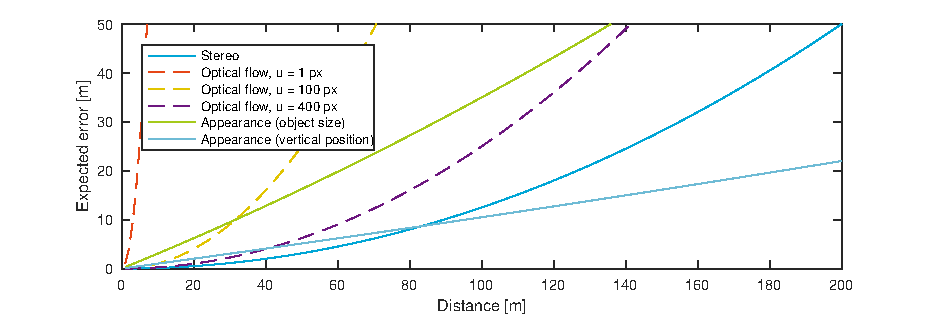
\includegraphics{range_comparison.pdf}
\caption{Comparison of expected error bounds for selected depth estimation methods.}
\label{fig:depth_comparison}
\end{figure}

\begin{table}
\centering
\begin{tabular}{lr}
\toprule
$B$ & \SI{20}{\centi\m} \\
$f$ & \SI{400}{\px} \\
$\dot z$ & \SI{10}{\m\per\s} \\
$\Delta t$ & \SI{0.1}{\s} \\
$L$ & \SI{10}{\m} \\
$A$ & \SI{100}{\m} \\
\midrule
$\epsilon_d$ & \SI{0.1}{\px} \\
$\epsilon_{\Delta u}$ & \SI{1.0}{\px} \\
$\epsilon_l$ & \SI{2}{\px} \\
$\epsilon_L$ & \SI{3}{\m} \\
$\epsilon_A$ & \SI{10}{\m} \\
\bottomrule
\end{tabular}
\caption{Parameters used to generate \autoref{fig:depth_comparison}. Error bounds $\epsilon_l$, $\epsilon_L$ and $\epsilon_A$ are an educated guess, the bounds $\epsilon_d$ and $\epsilon_{\Delta u}$ are based on literature and the KITTI benchmark.}
\label{tab:depth_params}
\end{table}

\subsection{Avoidance}
\label{sec:avoidance}
When an obstacle is detected along the \ac{UAV}'s direction of travel, it should perform an avoidance maneuver to prevent a collision.
There are different ways to handle this, from the very simple and lightweight reflexive behaviors, to high-level planning in maze-like environments.

The execution of an avoidance maneuver typically requires the following components: 1) \emph{motion planning}, which determines the actions the \ac{UAV} should take; 2) a \emph{map}, a representation of the obstacles in the vicinity of the \ac{UAV} and 3) \emph{odometry}, which is often required to accurately perform the planned maneuver.
These components will be briefly discussed in the following subsections.

\subsubsection{Motion planning}
Motion planning determines the action the \ac{UAV} should take to avoid collisions while moving towards its goal location.
An overview of motion planning and obstacle avoidance algorithms can be found in \cite{Goerzen2010,Minguez2016}.

\citeauthor{Minguez2016} \cite{Minguez2016} make a distinction between global planning and local planning (called `motion planning' and `obstacle avoidance' in their article, these terms will not be used here to avoid confusion with the overall task of obstacle avoidance).
\emph{Global planning} assumes that the location of all obstacles is known, the goal is to find a trajectory that optimizes a given performance measure.
\emph{Local planning} assumes that only obstacles detected by the \ac{UAV}'s sensors are known.
The goal here is to adapt the current trajectory of the \ac{UAV} to avoid a collision with nearby obstacles.
Local planning has the disadvantage that it can get trapped in certain situations (mazes for example, but these situations are unlikely in outdoor flight).
However, unlike global planning it can function in unknown environments.
Local planning is therefore the most relevant for \ac{UAV} obstacle avoidance.

Motion planning algorithms can be broadly divided into the following classes: reactive planning, planning without dynamics and planning with dynamics.
\emph{Reactive planning} refers to a class of algorithms that prescribe a control input or motion based directly on the presence of obstacles.
An example is the use of potential fields to determine the direction of travel of the \ac{UAV}: detected obstacles `repel' the drone, preventing a collision.
In \emph{planning without dynamics} the goal is to find a path for the \ac{UAV} that guides it past the detected obstacles.
This path should also minimize a cost function, setting these algorithms apart from reactive planning.
Once a path is found, it is left to a lower-level controller to actually follow it.
An example is \cite{Matthies2014} where a \ac{RRT} is used to plan a path through a forest.
\emph{Planning with dynamics} also optimizes a cost function, but includes a dynamic model of the \ac{UAV}.
\ac{MPC} is an example of this.
The inclusion of dynamics ensures that the maneuver can actually be performed, but requires a dynamic model of the \ac{UAV} to be available.
The use of dynamics is particularly suitable for high-performance manneuvers (e.g. drone racing), while planning without dynamics is more suitable for general-purpose applications as it does not require a model.

For brevity this section only lists examples of algorithms.
The reader is referred to the cited reviews for a more extensive overview of methods.



\subsubsection{Maps}
\label{sec:maps}
Motion planning requires a map, but the exact function of the map differs per algorithm.
At the very least, the map serves to document the location of nearby obstacles; even reactive planning will need this information.
For more complicated algorithms, the map allows the planning of an avoidance maneuver around the obstacles.
Finally, a map allows multiple observations of obstacles to be combined, which is the basic idea behind \ac{SLAM}.

Maps can be made at different levels of detail.
Ground robots and autonomous cars often create highly detailed maps of their immediate surroundings.
These types of maps are also applicable to \acp{UAV} flying at low altitudes or indoors, but their creation is computationally intensive.
An example of less detailed maps for aircraft is the \acf{EGPWS}, which uses relatively coarse-scaled static maps to prevent terrain collisions on passenger aircraft.
Such a map could also be used on \acp{UAV} as a form of geofencing, but this would primarily apply to cruise flight as such a static map is difficult to keep up to date at a high enough level of detail for take-offs and landings.

\begin{table}
\centering
\caption{Overview of common properties of map types. This table only lists the typical properties of these maps; exceptions can likely be found for many entries in this table. Note that combinations of these maps are possible (e.g. a cartesian voxel map for static obstacles and an \acs{EKF} for the positions of other aircraft).}
\label{tab:maps}
\let\oldfootnoterule\footnoterule
\renewcommand\footnoterule{\vspace{-0.5em}}
\begin{minipage}{\textwidth}
\small
\begin{tabular}{llllll}
\toprule
& Image-space & \multicolumn{2}{l}{Discretized space (voxels)} & \multicolumn{2}{l}{Continuous space} \\
\cmidrule(lr){3-4} \cmidrule(lr){5-6}
&& Cartesian & Polar & Point cloud & Obstacle positions \\
\midrule
Computational complexity & Low & High & High & High & Low \\
Volumetric & 2.5D\footnote{Volumetric in horizontal and vertical directions but not in depth.} & Yes & Yes & No\footnote{It is possible to fit a mesh on the point cloud or assume a small, fixed volume around each point.} & No\footnote{A fixed volume can be assumed for the obstacle, if known.} \\
Probabilistic & No & Occupancy & Occupancy & Position & Position \\
Dynamic & No & No & No & Yes & Yes \smallskip\\
Single-frame & Yes & Yes & Yes & Yes & Yes \\
Multi-frame & No & Yes & No & Yes & Yes \\
Reference frame & Body & World & Body & Any & Any \\
\bottomrule
\end{tabular}
\end{minipage}
\renewcommand\footnoterule{\oldfootnoterule}
\end{table}

Table \ref{tab:maps} lists map types that could be used to model the immediate surroundings of the \ac{UAV} during flight.
The maps are divided into three classes: image-space maps, discretized space maps and continuous space maps.
\emph{Image space} maps are essentially the same as depth maps: they consist of pixels for which the distance towards the first obstacle is stored.
\emph{Discretized space} maps split the surroundings of the drone into a collection of discrete cells that can be free or occupied.
These maps are commonly used for range-sensor-based \ac{SLAM} on indoor robots.
Finally, \emph{continuous space} maps do not discretize the space around the \ac{UAV}, but store a continuous position estimate for each measurement point.
A point cloud is a typical example of this map, but it is also possible to track the position of entire objects.

Table \ref{tab:maps} compares common properties of these map types.
In principle all of these maps can successfully be used on \acp{UAV}, but it depends on the application which map is the most suitable.
The most important decision is whether the map should combine multiple measurements or represent only a single measurement.
Combining multiple measurements allows the drone to map large and complex environments; it is therefore particularly suited for indoor operations but its use is limited to larger drones as the underlying algorithms can be computationally intensive.
Cartesian voxel maps are a common choice for this application (e.g. \cite{Schmid2014,Marzat2017}).
If the environment is simple enough that it can be captured in a single measurement, then image-space maps are a logical choice as these require very little processing to create and because other map types do not provide additional advantages if they do not fuse multiple measurements.
An example of the use of an image-space map for \ac{UAV} obstacle avoidance is found in \cite{Matthies2014}.
For the avoidance of other aircraft, a continuous-space map is a good choice as such a map is easy to update and can also model the velocity of the other aircraft.
An \ac{EKF} with the states of the detected aircraft is an example of such a map.






\subsubsection{Odometry}
\label{sec:odo}
To perform all but the most basic avoidance maneuvers, the \ac{UAV} will need an estimate of its velocity.
Outdoors \ac{GPS} is often available, but reflections can make it inaccurate in densely built areas.
Indoors, \ac{GPS} is not available for navigation so a different solution needs to be found.

A common solution for \ac{GPS}-less flight is \acf{VO}, where a camera is used to estimate the velocity of the drone.
The simplest methods directly transform the optical flow from a bottom-facing camera into a velocity estimate; this is commonly combined with sonar measurements to provide a sense of scale.
More complex \ac{VO} algorithms are closely related to \ac{SLAM} but lack loop closure capabilities.
These algorithms often estimate the \ac{UAV}'s pose relative to a \emph{keyframe}.
The use of a keyframe instead of the integration of velocities prevents drift over time; errors only accumulate when new keyframes are created.

\ac{VO} algorithms can be separated into dense and sparse algorithms, and direct and indirect methods.
A good description of these categories is provided in the introduction of \cite{Engel2017}.
The dense and sparse attributes are similar to those in stereo vision and optical flow: sparse algorithms only track a small number of keypoints, while dense algorithms use the entire input image.
Direct and indirect refers to the way that keypoints are matched or tracked: direct methods rely only on the intensities of neighboring pixels, while indirect methods first need to construct feature descriptors.

Both monocular, stereo and RGB-D vision can be used for \ac{VO}.
Stereo and RGB-D have the advantage that the map can be initialized from a single observation; this is not the case for monocular \ac{VO} as one observation can only provide the bearing of the keypoints.
Since a depth map is already required for obstacle avoidance, it should also be used for \ac{VO}.

Another design consideration is the use of an \ac{IMU}.
\acp{IMU} measure accelerations and angular velocities, which can be integrated to track the drone's pose.
Additionally, it can provide an estimate of the gravity vector.
The \ac{IMU} typically has a higher update rate than the camera and is also not sensitive to the appearance of the environment.
The integration of small measurement errors, however, causes the pose estimate to drift over time -- especially in the horizontal plane \cite{Woodman2007}.
It is therefore not practical to rely on solely the \ac{IMU}, it needs to be fused with other measurements like \ac{VO}.
There are two approaches to the fusion of \ac{IMU} data with \ac{VO}: tight coupling and loose coupling.
With tight coupling, the \ac{IMU} measurements are used in the same filter that performs the visual pose estimation, for instance in the update step of an \ac{EKF}.
With loose coupling, the vision-based pose estimate is calculated separately, after which a second filter is used to fuse it with the \ac{IMU} measurement.
Tight coupling produces more accurate results, but loose coupling might be easier to implement with existing autopilot filters.
A second use of the \ac{IMU} is in feature tracking.
The \ac{IMU} can be used to predict the next position of keypoints; this estimate can reduce the search space for tracking.
An example of this principle can be found in \cite{Sanfourche2013}.

An overview of \ac{VO} methods is presented in \autoref{tab:vo}.
\ac{UAV} obstacle avoidance applications should prefer methods that use stereo or RGB-D input together with the \ac{IMU}.

\begin{sidewaystable}
\centering
\hspace{-3cm}
\caption{Overview of \ac{VO} algorithms.}
\label{tab:vo}
\begin{tabular}{lp{3cm}lllp{5cm}p{5cm}}
\toprule
\textbf{Method} & \textbf{Camera} & \textbf{IMU} & \textbf{S/D} & \textbf{Descriptor} & \textbf{Code available} & \textbf{Platform} \\
\midrule
DSO \cite{Engel2017} & Mono & -- & Sparse & Direct & \url{https://github.com/JakobEngel/dso} & CPU, laptop $5\times$ real-time \\
SVO2 \cite{Forster2017} & Mono (incl. fisheye, catadioptric), stereo & Yes (optional) & Sparse & Direct & Binary only, incl. armhf. \url{http://rpg.ifi.uzh.ch/svo2.html} & Laptop, smartphone (100fps), \acs{MAV} \\
ORB-SLAM2 \cite{Mur-Artal2017} & Mono, stereo, RGB-D & -- & Sparse & ORB & \url{https://github.com/raulmur/ORB_SLAM2} & Core i7 real-time \\
\citeauthor{Usenko2016} \cite{Usenko2016} & Stereo & Yes & Semi & Direct & -- & -- \\
OKVIS \cite{Leutenegger2015} & Mono, stereo & Yes & Sparse & BRISK & \url{https://github.com/ethz-asl/okvis} & Real-time (platform not mentioned) \\
ORB-SLAM \cite{Mur-Artal2015} & Mono & -- & Sparse & ORB & \url{https://github.com/raulmur/ORB_SLAM} & -- \\
ROVIO \cite{Bloesch2015} & Mono & Yes & Sparse & Direct & \url{https://github.com/ethz-asl/rovio} & CPU 1-core 33fps \\
SVO \cite{Forster2014} & Mono & No & Sparse & Direct & \url{https://github.com/uzh-rpg/rpg_svo} & Embedded on MAV 55fps, Laptop 300fps \\
\citeauthor{Schmid2014} \cite{Schmid2014} & Stereo & Yes & Sparse & Direct & -- & \acs{MAV} \\
LSD-SLAM \cite{Engel2014,Engel2015} & Mono (incl. fisheye, catadioptric), stereo & No & Dense & n/a & \url{https://github.com/tum-vision/lsd_slam} (without stereo support) & CPU $40\times$ real-time \\
eVO \cite{Sanfourche2013} & Stereo & Gyro only & Sparse & Direct & -- & CPU \SI{1.86}{\mega\Hz} 2-core $12-\SI{56}{\milli\s}$ per frame \\
DVO \cite{Kerl2013} & RGB-D & Yes (optional) & Dense & n/a & \url{https://github.com/tum-vision/dvo_slam} & CPU 1-core 30fps \\
MSCKF 2.0 \cite{Li2013} & Mono, stereo & Yes & Sparse & Direct & \nth{3}-party implementations on github & CPU i7 \SI{2.66}{\giga\Hz} 1-core \SI{10}{\milli\s} per frame \\
DTAM \cite{Newcombe2011} & Mono & -- & Dense & n/a & openDTAM & GPU \\
PTAM \cite{Klein2007} & Mono & -- & Sparse & Direct & \url{http://www.robots.ox.ac.uk/~gk/PTAM/} & -- \\
\bottomrule
\end{tabular}
\end{sidewaystable}



\subsection{Performance evaluation}
\label{sec:perf}
Once a \acf{CAS} has been implemented, its performance should be evaluated.
The literature review on this subject can be kept brief: hardly any literature exists on this topic.
Most articles on obstacle avoidance demonstrate their method in an example application, but there is no common benchmark on which they can be compared.

A first step towards such a benchmark was taken in \cite{Nous2016}.
One of the core ideas of this paper is that the obstacle avoidance task can be split into smaller subtasks that can be evaluated independently.
For instance, the accuracy of obstacle detection can be evaluated independently from the \ac{UAV}'s motion planning algorithm or state estimator.

The main difficulty in the development of a benchmark is to find suitable metrics to describe the avoidance problem: the metrics should be chosen such that different environments with the same metrics (e.g. obstacle density, typical obstacle size) result in the same behavior.
It should be possible to predict the performance of an obstacle avoidance system when all relevant metrics of the target environment are available.
Such a benchmark would be extremely valuable both for \acp{UAV} and other types of robots.

A similar lack of benchmarks exists for robot navigation.
A proposal for a navigation benchmark is found in \cite{Sprunk2015}, perhaps this paper can also serve as inspiration for an obstacle avoidance benchmark.
